\begin{figure}[!tbh]
  \resizebox{\linewidth}{!}{
    \centering
    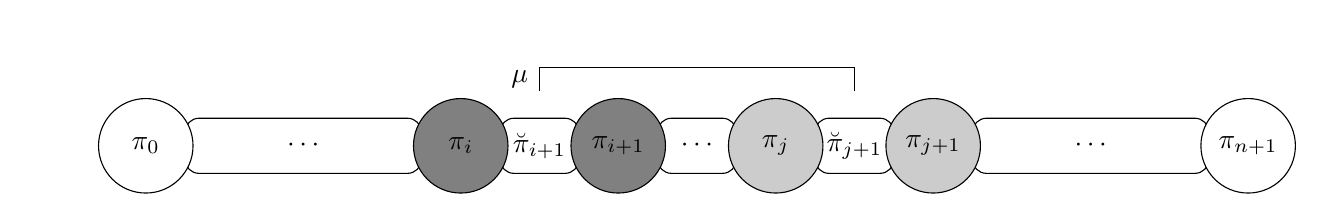
\begin{tikzpicture}
      %%%%% e)

      \node[draw=none,fill=none, minimum height=1cm, minimum width=1cm] at (-3.0, -11.0) {};

      % intergenic regions
      \node[rectangle,draw,fill=white!20, minimum height=.7cm, minimum width=3cm, rounded corners=5pt] at (0.0, -12.0) {$\cdots$};
      \node[rectangle,draw,fill=white!20, minimum height=.7cm, minimum width=1cm, rounded corners=5pt] at (3.0, -12.0) {$\breve\pi_{i+1}$};
      \node[rectangle,draw,fill=white!20, minimum height=.7cm, minimum width=1cm, rounded corners=5pt] at (5.0, -12.0) {$\cdots$};
      \node[rectangle,draw,fill=white!20, minimum height=.7cm, minimum width=1cm, rounded corners=5pt] at (7.0, -12.0) {$\breve\pi_{j+1}$};
      \node[rectangle,draw,fill=white!20, minimum height=.7cm, minimum width=3cm, rounded corners=5pt] at (10.0, -12.0) {$\cdots$};

      % genes
      \node[draw, circle, minimum height=1.2cm, minimum width=1.2cm, fill=white!20] at ({(2*0 - 2)}, -12.0) {$\pi_{0}$};
      \node[draw, circle, minimum height=1.2cm, minimum width=1.2cm, fill=black!50] at ({(2*2 - 2)}, -12.0) {$\pi_{i}$};
      \node[draw, circle, minimum height=1.2cm, minimum width=1.2cm, fill=black!50] at ({(2*3 - 2)}, -12.0) {$\pi_{i+1}$};
      \node[draw, circle, minimum height=1.2cm, minimum width=1.2cm, fill=black!20] at ({(2*4 - 2)}, -12.0) {$\pi_{j}$};
      \node[draw, circle, minimum height=1.2cm, minimum width=1.2cm, fill=black!20] at ({(2*5 - 2)}, -12.0) {$\pi_{j+1}$};
      \node[draw, circle, minimum height=1.2cm, minimum width=1.2cm, fill=white!20] at ({(2*7 - 2)}, -12.0) {$\pi_{n+1}$};

      % indexes
      \draw (3.0, -11.3) -- (3.0, -11.0);
      \draw (7.0, -11.3) -- (7.0, -11.0);
      \draw (3.0, -11.0) -- (7.0, -11.0);
      \node[draw=none,fill=none] at (2.75, -11.15) {$\mu$};
    \end{tikzpicture}
  }
  \caption[Exemplo de remoção de pelo menos um breakpoint tipo um após a aplicação de um move $\mu$.]{Exemplo de remoção de pelo menos um breakpoint tipo um após a aplicação de um move $\mu$.}
  \label{figure:CAIZFSWA}
\end{figure}